\documentclass{beamer}
%\begin{document}
\usepackage[utf8]{inputenc} % codificacao de caracteres
\usepackage[T1]{fontenc}    % codificacao de fontes
\usepackage[brazil]{babel}  % idioma
\usetheme{CambridgeUS}         % tema
\usecolortheme{orchid}      % cores
\usefonttheme[onlymath]{serif} % fonte modo matematico


% Set Color ==============================

% Custom colors
\usepackage{xcolor}
\usepackage{graphicx}

% http://www.computerhope.com/htmcolor.htm
\definecolor{gold}{HTML}{FDB525}
\definecolor{darkblue}{HTML}{294A75}
\definecolor{lightblue}{HTML}{62C7D1}
\definecolor{blue}{HTML}{0F96AC}

\makeatletter
\definecolor{mybackground}{HTML}{294A75}
\definecolor{myforeground}{HTML}{0000A0}

\setbeamercolor{normal text}{fg=black,bg=white}
%\setbeamercolor{alerted text}{fg=red}
%\setbeamercolor{example text}{fg=black}

%\setbeamercolor{background canvas}{fg=myforeground, bg=white}
%\setbeamercolor{background}{fg=myforeground, bg=mybackground}

\setbeamercolor{title}{bg=darkblue, fg=white}
\setbeamercolor{frametitle}{bg=darkblue, fg=white}

\setbeamercolor{palette primary}{fg=white, bg=blue}
\setbeamercolor{palette secondary}{fg=white, bg=lightblue}
\setbeamercolor{palette tertiary}{fg=black, bg=gold}
\setbeamercolor{palette quaternary}{fg=black, bg=darkblue}
\makeatother
% Set Color ==============================

\newcommand{\putat}[3]{\begin{picture}(0,0)(0,0)\put(#1,#2){#3}\end{picture}}

% Titulo
\title[Defesa de Mestrado]{Extensão do Bench4Q para \textit{benchmark} de desempenho em regime transiente}

\author[Flavio Souza]{Aluno: Flavio Luiz dos Santos de Souza \\ \and Prof. Dr. Francisco José Monaco}
\institute[ICMC-USP]{Instituto de Ciências Matemáticas e de Computação \\ Universidade de São Paulo} % opcional
\date{\today}
%============================================================================================

\begin{document}
 
\begin{frame}
  \titlepage
  
  \putat{195}{7}{
  	\includegraphics[scale=0.37]{images/lasdpc.png}
  }
  \includegraphics[scale=0.2]{images/USP_logo_icmc.jpg}

\end{frame}
 
 
\begin{frame}[allowframebreaks]{Sumário}
	\tableofcontents
\end{frame} 


%==================== INTRO
\section{Introdução}
Há poucos anos que a Computação em Nuvem deixou de ser um tema exclusivo de acadêmicos, hoje se faz presente na vida de pessoas e empresas muitas vezes passando-se despercebida em suas rotinas e atividades do cotidiano. Estabelecendo-se como uma importante e fundamental meio computacional. 

A Computação em Nuvem, é de fato um serviço em ebulição e que tem se tornando um paradigma cada vez mais reconhecido e utilizado. Inúmeras empresas têm apoiado e incentivado o uso e o seu desenvolvimento tão quanto no meio científico. Atualmente, os exemplos deste paradigma de computação possuem diversas opções para armazenamento ou processamento de dados, como, por exemplo, a \textit{\sigla{S3}{Simple Storage Service}} da Amazon, Bigtable do Google, ou PNUTS do Yahoo \cite{Binnig2009}. \citeonline{vazquez2014} exemplificam com o crescimento do Instagram, que construíram a sua base de usuários, de mais de 150 milhões de usuários, em menos de quatro anos usando soluções em nuvem.

O aumento da popularidade da computação em nuvem é impulsionado pelas vantagens oferecidas e pelo modelo dinamicamente escalável e o rápido desenvolvimento nos últimos anos levou a uma enorme quantidade de publicações. Embora ainda novo, o grande interesse no meio acadêmico e da indústria têm levado a uma quantidade considerável de publicações de artigos científicos nos últimos anos \cite{Heilig2014}. Como apresentado nos trabalhos de \citeonline{Heilig2014} e \citeonline{Yang2012}, o número de pesquisas têm concentrado esforços na resolução de problemas que em geral envolvem performance e/ou garantia de requisitos de Qualidade de serviço (\textit{\sigla{QoS}{Quality of service}}). 

A computação em nuvem tem emergido como um paradigma flexível de modo a facilitar a gestão de seus recursos e implementar aplicações elásticas em escala sem precedentes \cite{Cervino2012}. Existe uma grande preocupação por parte dos provedores de computação em garantir QoS de uma forma eficiente. Em termos de recursos, significa que os recursos virtuais (\textit{\sigla{VMs}{Virtual Machines}}) e/ou físicos tem devem ser alocados de forma autônoma, para que possam responder às influências externas, como a carga de trabalho. Em geral, os \textit{data center} são muitas vezes subutilizados devido ao excesso de provisionamento, bem como as demandas de recursos que variam no tempo de acordo com os sistemas \cite{Padala2007}. \citeonline{Inomata2011} afirmam que tempo e dinheiro são investido para projetar, construir, configurar, monitorar e manter recursos computacionais e que o futuro da computação em nuvem é o auto gerenciamento e a atribuição de recursos automáticos aos seus consumidores com base na carga de trabalho.

Atualmente, com o advento e crescimento das aplicações intensivas de dados, que lidam com grandes volumes em tempo real, a dinâmica do sistema passa ser perceptível e apreciável, fenômeno não perceptível claramente para os sistemas computacionais. Na prática, tais aplicações, de grande volume de dados, tendem a terem cargas de trabalho variante no tempo, causando inúmeros problemas imprevisíveis no sistema. A computação em nuvem oferece uma infraestrutura elástica ou escalável que pode ser utilizada para obter recursos \textit{on-demand}, no entanto, um problema em aberto é decidir sobre a correta alocação de recursos ao implantar na nuvem \cite{Cervino2012}. De modo geral, um sistema dinâmico não apresenta os efeitos das ações da carga de forma imediata. Como, por exemplo, a velocidade de um carro não muda imediatamente quando o pedal do acelerador é acionado e tão quanto menos uma temperatura em uma sala muda instantaneamente quando um aquecedor é ligado. Da mesma forma que uma dor de cabeça não desaparece logo após tomar uma aspirina, para todos os casos se requer tempo para que o efeito da ação se apresente resultado \cite{Karl2008}.

Este comportamento, dinâmico, começou a ser apresentado e apreciado em grande sistemas computacionais, como um súbito aumento de requisições para um \textit{website} onde os servidores não conseguem suportar a demanda. \citeonline{Arlitt2000} apresentam, um trabalho detalhado com os \textit{logs} de requisições do \textit{website} oficial da Copa do Mundo de Futebol do ano de 1998. Os dados foram coletados durante 3 meses e em 30 servidores distribuídos espalhados em 4 pontos do planeta. As requisições superaram a taxa de 1 bilhão, uma média de 11.000 requisições por minuto.

\begin{figure}[htb]
	\centering
	\includegraphics[scale=0.7]{log-world-98.png}
	\caption{Volume diário de tráfego para o Web Site Copa do Mundo}
	\label{fig:log98}		
	\fadaptada{Arlitt2000}
\end{figure}

A Figura \ref{fig:log98} apresenta o volume de requisições diária recebida pelo site Oficial da Copa do Mundo de 1998. No início de Maio até o início do evento (10 de junho) o volume de requisições são baixos em comparação ao início da Copa de 1998. A partir do dia 10 de Junho o volume de requisições cresce enormemente, este fenômeno é chamado de \textit{burstiness} (rajadas). O site de repente tornou-se muito popular devido ao início do evento e permaneceu por um longo período. O dia com maior volume de requisições foi 30 de Junho, quando mais de 73 milhões de requisições foram tratadas pelo site, após 30 de Junho os volumes de requisições diárias começam a diminuir lentamente até o final da Copa do Mundo, momento em que o volume de tráfego diminui rapidamente \cite{Arlitt2000}.

O \textit{burstiness} no fluxo de requisições são frequentemente encontrados em sistemas cliente-servidor. Esse \textit{burstiness} pode impactar de forma inesperada o desempenho de diferentes mecanismos de alocação de recursos projetados para o gerenciamento de um sistema adaptativo, e, portanto, testar e avaliar esses mecanismos sob cargas de trabalho reproduzíveis e controláveis é fundamental para o projeto do sistema.  Como ilustração, durante o evento promocional de \textit{e-commerce} conhecido como \textit{Black Friday}, na edição de 2012, foi constatado que o tempo de resposta médio aos dias que antecederam 23 de Novembro de 2012, era de 5.3 segundos. A partir das 7 horas do dia evento, observou-se um aumento significativo no tempo de resposta conforme apresentado no gráfico da Figura \ref{fig:grafico-black-friday}. Apesar de estar hospedado na \textit{Cloud Computing} (computação em nuvem) e ciente de que o volume de requisições aumentaria, não foi possível manter a qualidade de QoS, tempo de respostas, aos clientes.

Existem muitas abordagens em uso hoje para gerenciar recursos, abrangendo \textit{hardware} e \textit{software}. Ser capaz de medir o desempenho é fundamental para o trabalho da engenharia que busca melhorar as capacidades e a melhor utilização dos recursos.

\begin{figure}[htb]
	\centering
	\includegraphics[scale=0.45]{grafico-black-friday.jpg}
	\caption{Tempo de resposta do \textit{Black Friday} Brasil 2012}
	\label{fig:grafico-black-friday}
	\fadaptada{blackfridayNews}
\end{figure}

As técnicas de gerenciamento de recursos são inúmeras, como as de inteligência artificial que utilizam lógica \textit{fuzzy}, algoritmos de mineração de dados e aprendizado de máquina \cite{Nobile2013}. As técnicas de aprendizado de máquina mostram-se interessantes para soluções imediatas, onde não há tempo hábil, inclusive, com abordagens não lineares empregadas para implementar um gerenciador de recursos, responsável pela alteração dinâmica das capacidades computacionais. Outros trabalhos, como o \citeonline{Zhang2007}, buscam identificar padrões de comportamento na carga de trabalho e otimizam a provisão dinâmica de recursos nas máquinas virtuais com base em algoritmos reativos. Utilizando uma abordagem descentralizada e o modelos \textit{Box-Jenkins} de \citeonline{box2011} para particionamento de recursos. \citeonline{Quiroz2009} buscam detectar, por monitoramento, a padronização e a tendência da carga de trabalho com o objetivo de otimizar os recursos. \citeonline{Nobile2013} também propõe o uso de modelos de séries temporais para modelagem de tráfego de tempo real e previsão de demanda, que é usada para criar partições de conexões para diferentes classes de prioridade. Já \citeonline{Zhang2011}, afirma em seu trabalho, que a utilização de cada servidor nuvem varia de acordo com o tempo de execução, assim a temática de alocação de recurso e o balanceamento da carga de trabalho são desafios computação em nuvem. Logo, \citeonline{Zhang2011}, utiliza de técnicas de estatística e avaliação dos recursos disponíveis para tomar a decisão de qual recurso deve ser alocado.

%Afim de melhor aproveitamentos dos recursos disponíveis em um \textit{data center}, uma das técnicas utilizadas é a teoria de controle, que foi inicialmente proposto em 1960 para lidar com o controle de sistemas lineares invariantes no tempo com parâmetros desconhecidos, que agora alcança o objetivo de circuito fechado satisfatória especificado em termos de engenharia significativos quando a planta incerteza paramétrica é pequena. No entanto, as mudanças nas condições de funcionamento; falha ou degradação do componente; ou mudanças inesperadas na dinâmica do sistema pode tudo a pressuposição de incerteza pequeno, particularmente paramétrico incerteza. Os impactos mencionados acima sempre resultam em respostas de grandes e oscilatórios ou até mesmo instável, quando usando os métodos clássicos de controle adaptativo \cite{Narendra1997}. Essa técnica foi aplicada amplamente em diversas áreas da engenharia, sempre obtendo resultados positivamente satisfatórios e eficientes, até então pouco explorada na computação, os sistemas computacionais não sofriam de variações em seu trabalho, pois as variações nas aplicações eram praticamente imperceptíveis.
%Entretanto, essa técnica, teoria de controle, é pouco explorada e difundida nas áreas da computação mesmo não sendo recente e tento grandes sucessos em outra áreas. Esta técnica apresentar grande potencial de solução para diversos problemas em sistemas computacionais, como o problema de contenção na camada de enlace de dados para redes sem fio \cite{wang2008, boggia2007}.
%Não é de hoje que a teoria de controle tem sido muito bem aplicada e tendo resultados importantíssimos em diversas áreas da engenharia, sendo empregada como uma importante ferramenta na resolução de diversos problemas \cite{Ogata2001}. A evolução da Teoria de Controle na engenharia permitiu desenvolver uma gama de ferramentas de linguagem matemática que auxiliam na descrição de sistemas dinâmicos, como a resposta de diferentes estímulos. Apesar da presença da Teoria de Controle nas diversas áreas da engenharia, em sistemas computacionais é uma área a ser explorada e pesquisada na computação, e que tem ganhado cada vez mais espaço e atenção na área. Pesquisas recentes têm mostrado as possíveis aplicações da Teoria de Controle em sistemas computacionais de auto gerenciamento de recursos \cite{Nobile2013}. Como mostrado por \cite{Abdelzaher2008}, no gerenciamento de memória do IBM DB2, que gerencia a alocação de memória em tempo real, para resolver à variação da carga de trabalho, minimizando o tempo de resposta do sistema foi muito bem utilizada.

\citeonline{Dong2014} afirmam que atualmente, a maioria das aplicações Web são concebidas com sistemas \textit{mult-tiers} (multi-camadas), devido à flexibilidade de escalabilidade, o planejamento de capacidade é um método clássico para determinar a quantidade de recursos exigido para um determinado QoS. No entanto, o planejamento de capacidade é basicamente uma decisão de longo prazo e quase estático, e os recursos são determinados pela taxa de utilização máxima da aplicação para evitar a pena excessiva de QoS.

\citeonline{Lourenco2015} afirma que a partir de um planejamento de capacidade, a gestão de recursos em tempo real, aumenta a sofisticação da arquitetura da solução nos diversos níveis e complexidade, as abordagens convencionais para análise de sistemas computacionais modernos; e concluí que as dinâmicas emergentes das interligações desses sistemas \textit{mult-tiers} pode produzir efeitos transitórios sobre o desempenho, como resposta temporal, ou o amortecimento e/ou comportamento oscilatório. Uma vez que estes efeitos variáveis no tempo podem potencialmente afetar a capacidade de resposta, eficiência e até mesmo a estabilidade global, métodos e ferramentas para avaliação das propriedades dinâmicas de sistemas computacionais são de importância prática para fins da engenharia.

Outra técnica utilizada é a teoria de controle, que foi proposta em 1960 para lidar com o controle de sistemas lineares invariantes no tempo com parâmetros desconhecidos. Não é de hoje que a teoria de controle tem sido muito bem aplicada e tendo resultados importantíssimos em diversas áreas da engenharia, sendo empregada como uma importante ferramenta na resolução de diversos problemas \cite{Ogata2001}. A evolução da teoria de controle na engenharia permitiu desenvolver uma gama de ferramentas de linguagem matemática que auxiliam na descrição de sistemas dinâmicos, como a resposta de diferentes estímulos. Apesar da presença da teoria de controle nas diversas áreas da engenharia, em sistemas computacionais é uma área a ser explorada e pesquisada na computação, e que tem ganhado cada vez mais espaço e atenção na área. Pesquisas recentes têm mostrado as possíveis aplicações da técnica em sistemas computacionais de auto gerenciamento de recursos \cite{Nobile2013}. Como mostrado por \citeonline{Abdelzaher2008}, que estudou e aplicou uma abordagem controle de \textit{feedback} no contexto do gerenciamento de memória do \sigla{DB2}{\textit{Database Management System}} da IBM,  para gerenciar a alocação de memória em tempo real e responder a uma variação da carga de trabalho e minimizando o tempo de resposta do sistema.

Para facilitar o entendimento e lidar com sistemas grandes e complexos, é interessante ter maneiras de validar esses sistemas de modo a garantir o desempenho sem prejudica o QoS. O desempenho de um sistema computacional pode ser medido por meio de técnicas de avaliação de desempenho, sendo assim, existem duas possibilidades básicas de abordagem: modelagem e aferição \cite{Jain1991}.

A teoria de controle utiliza da modelagem, um modelo que é uma representação matemática de um sistema físico, biológico ou de informação, esses modelos nos permitem raciocinar sobre um sistema e fazer previsões sobre como ele se comportará \cite{Karl2008}. Este trabalho está interessado principalmente em modelos de sistemas dinâmicos que descrevem o comportamento de sistemas de entrada e saída. De modo geral um sistema dinâmico não apresenta os efeitos das ações imediatamente quando ocorrem. %Como por exemplo, a velocidade de um carro não muda imediatamente quando o pedal do acelerador é acionado e tanto quanto menos uma temperatura em uma sala muda instantaneamente quando um aquecedor é ligado. Da mesma forma, que uma dor de cabeça não desaparece logo após tomar uma aspirina, para todos os casos se requer tempo para que o efeito da ação se apresente \cite{Karl2008}.

Há caso em que existe o interesse em controlar a dinâmica deste sistema, para tanto é necessário modelar o sistema em questão e projetar um controlador que manipulará a sua dinâmica. Para trabalhar com estes sistemas deve-se ser capaz de modelar um sistema dinâmico, que em termos matemáticos é extrair um modelo matemático e analisar suas características dinâmicas. Um modelo matemático de um sistema dinâmico é definido como um conjunto de equações que representa a dinâmica de maneira relativamente razoável. Percebe-se que um modelo matemático não é exclusivo para um determinado sistema. Um sistema pode ser representando de muitas maneiras diferentes e, por conseguinte, podem ter diversos modelos matemáticos, dependendo da perspectiva, uns mais precisos que outros, e outros mais simplificados \cite{Ogata2001}.

Em geral, é possível representar sistemas dinâmicos através de equações diferenciais obtidas com base nas leis básicas da Física. Esses sistemas de equações diferenciais descrevem uma determinada dinâmica do sistema no domínio do tempo e, com o desenvolvimento dessas equações, é possível identificar propriedades fundamentais do sistema \cite{Nobile2013}.


A avaliação por aferição, medição direta via instrumentação apropriada, adequa-se muito bem as necessidade, no entanto, é necessário a existência e disponibilidade do sistema ou protótipo, pois a avaliação é feita através de estímulos às entradas (\textit{benchmark}) e leitura de suas saídas, possibilitando testes de caixa preta onde não é exigido conhecimento sobre o funcionamento interno do sistema, possibilitando a aquisição de resultados precisos devido à aplicação em sistema real \cite{Nobile2013}, como em um sistema dinâmico, no qual o comportamento do sistema evolui com o tempo, em resposta a estímulos externos.

Independente da abordagem, aferição ou modelagem, o importante da técnica de avaliação utilizada é a abrangência mediante ao comportamento em condição estática e dinâmica do sistema \cite{helder2014}.


\section{Motivação}

Embora amplamente aplicada e difundida em diversas áreas da engenharia e ciência, a avaliação de desempenho em regime transitório é pouco explorada e usada em sistemas computacionais, possivelmente está relacionado habituais e tradicionais sistemas computacionais, onde não é possível perceber a dinâmica do mesmo. Aplicativos móveis, \textit{notebooks} e \textit{\sigla{PCs}{Personal Computers}} estão criando cada vez maior capacidade computacional, que estimulam os sistemas enriquecidos de serviços, como entretenimento de mídia e redes sociais, jogos, etc. Emergindo e apresentando a dinâmica do sistema e despertando o interesse na análise transiente em sistemas computacionais, que ocorre concomitantemente ao aparecimento de aplicações, assim como os sistemas mecânicos ou elétricos que apresentam propriedades de inercia na transformação de estímulos (entrada) em resposta (saída) onde a dinâmica dos mecanismos constituintes se torna não negligenciável. É o caso de sistemas distribuídos de larga escala, de grande complexidade e envolvendo a interação pervasiva com sistemas físicos \cite{Egami2011, Kannan2011}. 

Neste contexto de pesquisa, o \textit{\sigla{LaSDPC}{Laboratório de Sistemas Distribuídos e Programação Concorrente}}\footnote{\url{http://www.lasdpc.icmc.usp.br}}, onde desenvolve este projeto, trabalhos anteriores lidam com essa temática, como o trabalho de \citeonline{Nobile2013}, que apresentou resultados que valorizam e apreciam os impactos no desempenho de um sistema com características dinâmicas, hospedado em um ambiente de computação em nuvem de recursos elásticos e com mecanismos de provisão de QoS, através da modelagem das propriedades de resposta transiente do sistema que são aplicadas e gerenciadas com  técnicas de teoria de controle. Em outro trabalho, \citeonline{Lourenco2015} apresentou uma especificação de uma arquitetura conceitual que separa responsabilidades de simulação dinâmica em um conjunto de preocupações básicas, e formaliza um modelo de referência abstrata para a concepção de ferramentas de simulação. Junto a instância da classes abstratas e implementadas algumas políticas de controle básicos e com o modelo podem ser facilmente utilizados em experimentos de simulação com o CloudSim. O trabalho de \citeonline{Edwin2015}, em desenvolvimento também no LaSDPC, estuda e define uma metodologia de análise transiente dedicado a sistemas computacionais dinâmicos reais utilizando da especificação arquitetural proposto por \citeonline{Lourenco2015}. A principal contribuição pretendida é a formulação e definição de uma metodologia para seu emprego em sistemas, cuja a metodologia deverá ser capaz de descrever e especificar os passos para modelar o sistema, projetar um controlador e analisar os resultados transiente mediante as variações na carga de trabalho. Para tanto, o trabalho de \citeonline{Edwin2015} utiliza de um \textit{benchmark} para a validação experimental de sua metodologia. No entanto, o \textit{benchmark} escolhido por \citeonline{Edwin2015}, Bench4Q, não contempla das especificações apresentadas por \citeonline{Lourenco2015}.

Segundo \citeonline{Binnig2009} os \textit{benchmarks} tradicionais não são suficientes para a análise desses novos serviços de elasticidade da computação em nuvem. O principal desafio dos novos \textit{benchmarks} é fazer com que os resultados apresentados, ou seja as métricas, ofereçam informações relevantes a esses diferentes serviços e com diferentes capacidades e garantias desses serviços. \citeonline{Dong2014} afirmam que, a maioria das aplicações Web são concebidas como sistemas \textit{mult-tiers}, devido à flexibilidade e capacidade de reutilização de \textit{software}, porem é difícil de modelar o comportamento de aplicações Web de \textit{multi-tiers}, devido ao fato de que a carga de trabalho estimula a dinâmica do sistema nos diferentes níveis da camada.

No âmbito da análise de desempenho em sistemas computacionais, definimos o \textit{benchmarking} como o ato de medir e avaliar o desempenho computacional, protocolos de rede, dispositivos e redes, sob condições de referência, em relação a uma avaliação de referência. O objetivo deste processo de \textit{benchmarking} é permitir a comparação equitativa por diferentes soluções, ou entre desenvolvimentos subsequentes de um \textit{\sigla{SUT}{\textit{System Under Test}}}. \textit{Benchmarking} é o principal método para medir o desempenho de uma máquina ou sistema. O \textit{benchmarking} refere-se à execução de um conjunto de programas representativos em diferentes computadores e redes, medindo os resultados. Esses resultados são utilizados para avaliar o desempenho de um determinado sistema com uma carga de trabalho bem definida \cite{Menasce2001}.

Entretanto, não existe aparato ferramental para a exploração dessas técnicas, apesar de existir diversos \textit{benchmarks} e ferramentas para o estudo, nenhuma delas estimulam a dinâmica transiente do sistema e permitem uma avaliação em regime transiente, que se faz necessário para a pesquisa de \citeonline{Edwin2015}. A proposta deste trabalho é identificar um \textit{benchmark} e adequá-lo de maneira em que estimule a dinâmica do sistema possibilitando uma avaliação transiente.


\section{Objetivo}
Este trabalho tem por objetivo a extensão de um \textit{framework} do \textit{benchmark} Bench4Q afim de atender os requisitos do modelo \textit{\sigla{MEDC}{\textit{Monitor, Effector, Demanda and Capacity}}}, proposto por \citeonline{Lourenco2015}. O objetivo restringe ao modulo de modulação da carga de trabalho, gerado pelo \textit{benchmark}, acrescendo-o de provisões nativas para gerar perturbações capazes de excitar e produzir o regime transiente do sistema SUT do \textit{benchmark}, onde poderá ser apreciado a sua dinâmica. A contribuição almejada é a disponibilização de um \textit{benchmark} que auxilie a análise de sistemas dinâmico e que possibilite a analise transiente do mesmo. São consideradas perturbações configuráveis na carga de trabalho, e resultados são apresentados pelo \textit{benchmark}.




%==================== REVISAO 
\section{Revisão}
\begin{frame}{O comportamento dinâmico em sistema físico}
	\begin{figure}[htb]
		\centering
		\includegraphics[scale=0.4]{../monograph/images/grafico-chaleira.png}	
		\caption{Dinâmica e comportamento da chaleira aquecendo \cite{Janert2013}}
	\end{figure}
\end{frame}

\begin{frame}{O comportamento dinâmico em sistema físico}
	\begin{figure}[htb]
		\centering
		\includegraphics[scale=0.4]{../monograph/images/grafico-mola.png}	
		\caption{Dinâmica e comportamento da mola \cite{Janert2013}}
	\end{figure}
\end{frame}

\begin{frame}{Revisão}
	
	\begin{figure}[!htb]
		\centering 
		\includegraphics[scale=0.33]{images/abstracao-nobile2.png}
		\caption{Metodologia usada por \cite{Nobile2013}.}
		\label{fig-market-oriented-broker}
	\end{figure}
	
\end{frame}

\begin{frame}{Estratégia Adaptativa}
	
	\begin{figure}
		\center
		\includegraphics[scale=0.3]{images/feedback-loop-3.pdf}
		\caption{Arquitetura de controle usada por \cite{Nobile2013}.}
		\label{fig:loop-nobile}
	\end{figure}
	
	\begin{itemize}
		\item \textbf{G:} \textit{Datacenter}.
		\item \textbf{H:} Sensor de retroalimentação.
		\item \textbf{C:} Controlador.
		\item \textbf{x:} Número de máquinas virtuais (sinal de controle).
		\item \textbf{o:} Taxa de utilização total (\textbf{y:} taxa relativa).
		\item \textbf{d:} Perturbações (picos de carga, \textit{backups}, etc.) 
		\item \textbf{r:} Entrada de referência da taxa de utilização.
	\end{itemize}
\end{frame}

\begin{frame}{Resultados}
	
	\begin{figure}
		\center
		\includegraphics[scale=0.65]{images/resposta-nobile.pdf}
		\caption{Taxa de utilização \cite{Nobile2013}.}
		\label{fig:taxa-nobile}
	\end{figure}
	
\end{frame}

\begin{frame}{Conclusão de \cite{Nobile2013}}
	
	Segundo \cite{Nobile2013}, a \textbf{modelagem das propriedades dinâmicas} e a \textbf{aplicação de técnicas de teoria de controle} em ambientes de recursos elásticos tem impacto apreciável. 
\end{frame}





%==================== MEDC
\section{MEDC}
\begin{frame}{Estudo de análise em regime transitório}
	\begin{itemize}
		\item \cite{Lourenco2015} discutem a abordagem de análise de estado estacionário vigente para avaliação de desempenho de sistemas computacionais
		
		\item apresenta um planejamento de experimentos de simulação destinados a análise transitória, especialmente em aplicações \textit{multi-tiers}.
	\end{itemize}
\end{frame}

\begin{frame}{Arquitetura conceitual MEDC}
	\begin{figure}
		\centering
		\includegraphics[scale=.4]{images/medc.png}
		\caption{MEDC: Monitor, Efetor, Demanda, Capacidade. \cite{Lourenco2015}}
		\label{fig:medc1}
	\end{figure}
\end{frame}

\begin{frame}{Modelo MEDC - o transiente}
	\begin{itemize}
		\item O transiente em um sistema computacional pode ser provocado por:
		\begin{itemize}
			\item Uma mudança na carga de trabalho 
			\item Uma mudança na capacidade interna (quantidade de recursos).
		\end{itemize}  
		\item O modelo MEDC mapeia esses dois aspectos nas responsabilidades respectivamente:
		\begin{itemize}
			\item \textbf{\textit{Demand} (modulação da carga)};
			\item \textit{Capacity} (modulação dos recursos).
		\end{itemize}
	\end{itemize}
\end{frame}



\begin{frame}{Modelo MEDC - demanda e capacidade}
	\note{no modelo MEDC diz que a ferramenta tem que incluir a pertubação de maneira programada realimentada (ex: quando a taxa de utilização ativem um nível)}
	\begin{itemize}
		%		\item O monitoramento produz as medidas para que a modulação de demanda e capacidade sejam feitas em tempo real;
		%		\begin{itemize}
		%			\item A saída do experimento deve produzir também gráficos temporais.
		%		\end{itemize}
		\item Uma perturbação pode ocorrer:
		\begin{itemize}
			\item Em função do tempo, (um acidente programado);
			\item Em função das medidas de desempenho, (de modo realimentado).
		
				\begin{itemize}
					\item \textbf{A modulação da carga} pode ser feita em função da \textit{taxa de requisições} (reduzir a carga admitida quando a utilização passar de certo limite).  
					\item \textbf{A modulação da capacidade} pode ser feita em função da utilização da CPU (aumentar os recursos quando a utilização ultrapassar certo patamar).  
				\end{itemize} 
		\end{itemize} 
	\end{itemize}
\end{frame}

%\begin{frame}{Modelo MEDC - Dinâmica}
%	\note{somente para completar o modelo, a capacidade e a demada dão os numeros mas quem atuaçõ é o Efector que é o mecanimos de atuação do Modelo}
%	\begin{itemize}
%		%		\item A modulação da demanda e a capacidade podem se refletir em: 
%		%		\begin{itemize}
%		%			\item política de admissão de carga;
%		%			\item gerenciamento de recursos.
%		%		\end{itemize} 
%		
%		\item A modelagem da dinâmica é responsabilidade do Efetor;
%		\begin{itemize}
%			\item O mecanismo pelo qual isso é implementado, fisicamente, pode \textbf{implicar em certa dinâmica}.
%			\item se a política de capacidade determina que os recursos devem ser aumentados, \textbf{o Efetor modela o atraso e a inércia} para a alocação e o desalocação dos recursos. 
%		\end{itemize}
%		
%	\end{itemize}
%\end{frame}



%\begin{frame}{O que é MEDC}
%	
%	\begin{columns}
%		\begin{column}{.4\textwidth}
%			\includegraphics[width=.85\linewidth,valign=t]{../monograph/images/extension-block.pdf}
%
%		\end{column}
%		\begin{column}{.6\textwidth}
%			\textbf{"um conjunto de requisito que especificam uma arquitetura conceitual, intitulada MEDC (\textit{Monitor, Effector, Demanda and Capacity})."}
%			
%			\hfill-- Lourenço 2015
%		\end{column}
%	\end{columns}
%		
%	%\vspace*{10pt}
%	\begin{columns}
%		\begin{column}{0.9\textwidth}
%			\begin{itemize}
%				\item[\textit{Demand}:] referência para a capacidade de entrada e determinar a forma como a carga de trabalho muda ao longo do tempo;
%
%				\item[\textit{Capacity}:]  é a disposição análoga no que diz respeito aos recursos do sistema;
%				
%				\item[\textit{Monitor}:] sensor e aquisição de dados temporais, coletando os dados sobre o sistema e torná-lo disponível;
%				
%				\item[\textit{Effector}:] mecanismos de atuação através modulação, serve para a modelar os componentes operacionais que afetam a dinâmica \textit{Capacity} e \textit{Demand}.
%			\end{itemize}
%		\end{column}
%	\end{columns}
%\end{frame}



%==================== BENCH4Q
\section{Bench4Q}
%==================== BENCH4Q
\begin{frame}{Bench4Q}

\begin{itemize}
\item Bench4Q e um \textit{benchmark} para avaliação de desempenho em regime estacionário.

\item Não existem provisões para a introdução de perturbações programadas durante o experimento.

\item Código fonte disponível~\footnote{http://www.trustie.net/projects/project/show/Bench4Q}.

\item Amplamente utilizado na literatura~\footnote{\cite{Wang2012b,Zhang2012a,Gao2013}}.
\end{itemize}


\end{frame}

\begin{frame}{Características}

Bench4Q:
\begin{itemize}
	\item É uma extensão do \textit{benchmark} \textbf{TPC-W} \cite{Garcia2003}.
	\item Suporta analise de métricas baseadas em sessões.
	\item A geração de carga é baseada em agentes:
	\begin{itemize}
		\item Cada agente disponibiliza vários \textit{Workers} ou EBs (\textit{Emulate Browsers}).
		\item Agentes locais ou remotos.
	\end{itemize}
	\item Utiliza uma loja de livros: \textit{Software Under Test} (\textbf{SUT}).
\end{itemize}

\end{frame}

\begin{frame}{Caraterísticas}
	\begin{figure}
		\begin{center}
			\includegraphics[scale=0.35]{images/sut.png}
			\caption{Bench4Q: SUT.}
			\label{fig:sut-bench4q}
		\end{center}
	\end{figure}
\end{frame}


\begin{frame}{Métricas disponíveis no Bench4Q}
%Métricas de interesse disponíveis no Bench4Q:
\begin{itemize}
	\item WIRT (\textit{Web Interaction Response Time})
	\item WIPS (\textit{Web Interacton Per Second})
	\item VSPS (\textit{Valid Sessions Per Second})
	\item VSR (\textit{Valid Sessions Ratio})	
\end{itemize}

\end{frame}

\begin{frame}{Métricas disponíveis no Bench4Q}
\begin{figure}
	\begin{center}
		\includegraphics[scale=0.5]{images/metricas.png}
			\caption{Bench4Q: Métrica VSPS.}
					\label{fig:vsps-bench4q}
	\end{center}
\end{figure}

\end{frame}

\begin{frame}{Arquitetura Bench4Q}
	\begin{figure}
		\begin{center}
			\includegraphics[scale=0.2]{images/bench4Q.png}
			\caption{Arquitetura Bench4Q \cite{Bench4Q}.}
			\label{fig:arquitetura-bench4q}
		\end{center}
	\end{figure}
\end{frame}

\begin{frame}{Gerador de carga}
  \putat{150}{-120,5}{
  	\includegraphics[scale=0.4]{images/console-bench4Q.png}
  }
\begin{itemize}
\item Tipos de navegação:
\begin{enumerate}
	\item \textit{Browsing}
	\item \textit{Ordering}
	\item \textit{Shopping}
\end{enumerate}
%\item Gerenciamento dos agentes.
\end{itemize}  


\end{frame}

\begin{frame}{Comportamento dos EBs}
CBMG (\textit{Customer Behavior Model Graph}) é um grafo estatístico que modela o comportamento de navegação de um usuário(emulado).

	\begin{figure}
		\center
		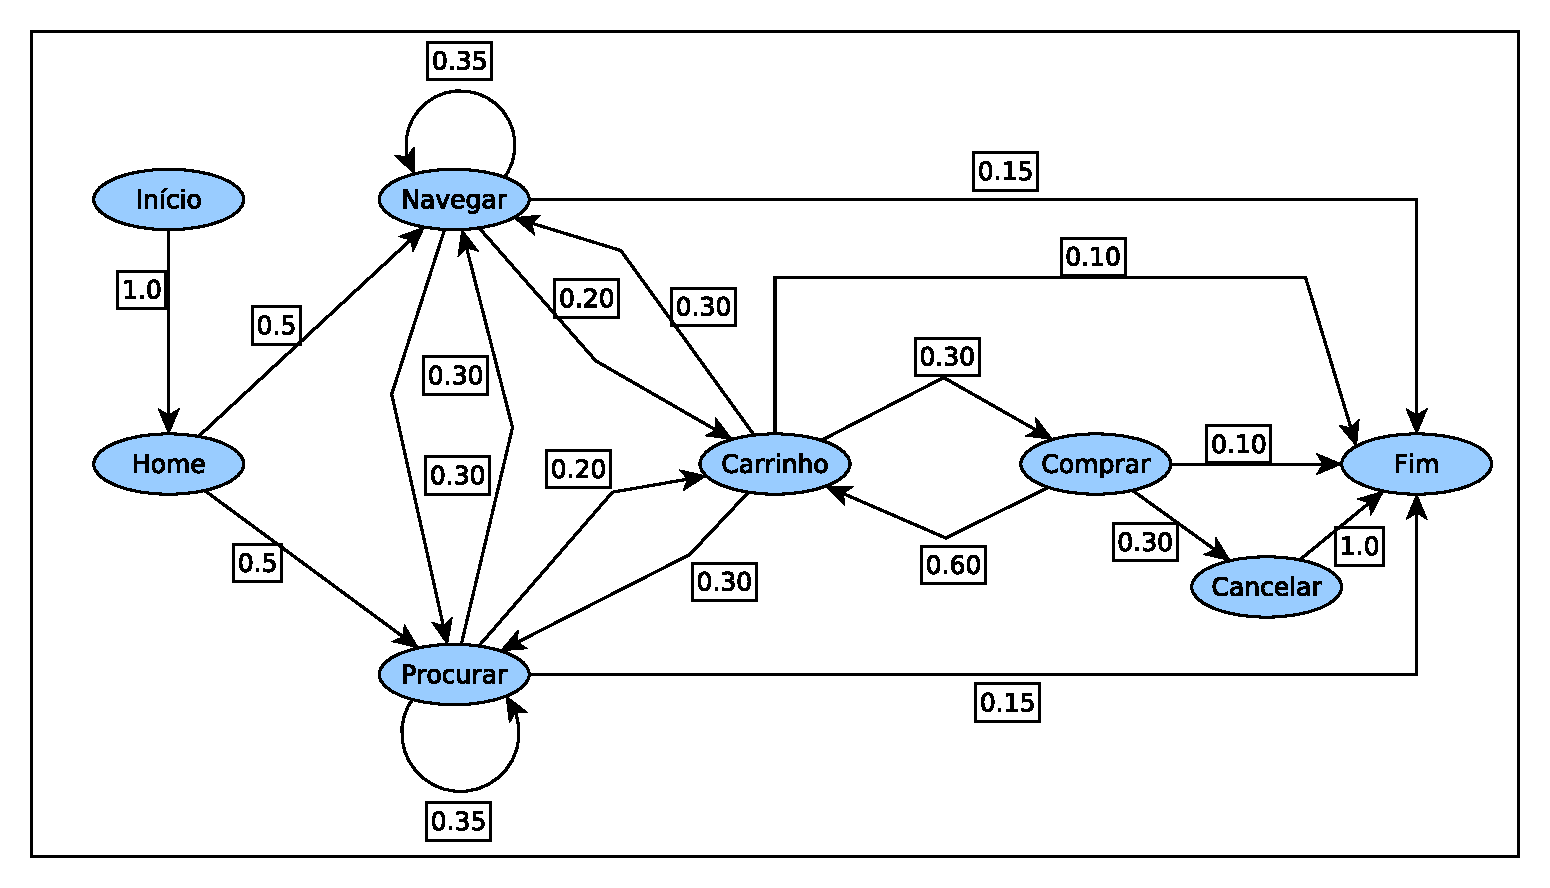
\includegraphics[scale=0.35]{images/CBMG}
		\caption{Perfil interação estocástico com o sistema (SUT).}
		\label{fig:CBMG}
	\end{figure}
\end{frame}

%==================== Metodologia
\section{Metodologia}
Existem diversos \textit{benchmarks} que especificam e simulam cargas de trabalho para avaliarem sistemas computacionais. No entanto, não existe nenhum \textit{benchmark} que possibilite uma avaliação em regime transiente. Este capítulo apresenta e defini uma metodologia de extensão de avaliação em regime transiente para \textit{benchmarks} aproveitando toda a sua maturidade e robustez.




\section{Estratégicas de extensão}

O \textit{benchmark} bench4Q define uma carga de trabalho, incluindo banco de dados, transações, regras de execução e de taxa de transferência e métricas de resposta.  Para expor a dinâmica de um sistema é necessário estimulá-lo, a carga de trabalho é quem estimulará o sistema através de cenários ou fenômenos de \textit{burstiness}. Essa implementação é composta por classes ou funções, influenciado diretamente pela linguagem em que o \textit{benchmark} foi desenvolvido, esse conjunto de código é um componente básico do \textit{benchmark} que refere-se a uma unidade de trabalho genérico que envia a carga para o sistema. Alguns \textit{benchmarks} incluem solicitações HTTP, chamadas de procedimento remoto, invocações de serviços Web, transações de banco de dados, comandos interativos ou também mesmo poderia ser composto de múltiplas tarefas de processamento, por exemplo sessões de cliente que compreendem várias solicitações ao sistema, etc \cite{Kounev2005}. Segundo \cite{Nobile2013} uma alteração na entrada (carga de trabalho) fará com que o sistema saia do estado em regime estacionário e entre em um período de regime transiente e para descrever a dinâmica de um sistema, comumente, o ganho em regime estacionário é calculado para uma entrada degrau unitário.

O objetivo deste trabalho é estender a carga de trabalho do sistema de tal maneira que permite-se estimular o sistemas a apresentar a sua dinâmica, assim possibilitando a analise transiente do sistema.


%Comumente a avaliação de desempenho de sistemas computacionais é realizada em regime estacionário, isto é, sob carga de trabalho constante. Tradicionalmente a avaliação feita dessa forma produz dados para inferir a capacidade estática do sistema. O sistema inicialmente sem carga, é excitado com a entrada de interesse, e aguarda-se até que a saída estabilize-se no valor desejado, podendo ser um valor constante ou um valor dentro de um intervalo. A condição aceitável é alcançada passado o warm up (aquecimento), período em que o sistema encontra-se em estado de inicialização. A determinação da capacidade obtém-se estimulando o sistema com carga gradativamente mais elevadas até atingir seu limite inferior de desempenho aceitável, correspondente à carga estática máxima suportada. Análise do comportamento no período de aquecimento contém informações importantes relacionadas com a capacidade do sistema operando em condições reais onde a carga não é constante.
%Em regime transiente, a quantidade de recursos necessários para garantir o desempenho especificado pode divergir substancialmente daquela definida em regime estacionário. Durante um período transiente, as consequências duma perturbação na carga a quantidade de recursos necessários seria temporariamente superior àquela prevista para o regime de carga não variável. Isso resulta, por exemplo, em descumprimento dos níveis de serviço ou paradas no funcionamento dos sistemas.
%Dentro de um ambiente de testes local uma das principais limitações na simulação de sistemas e-commerce é o acesso ao banco de dados. Percebe-se que o banco de dados é o principal fator limitante para a analise transiente  para níveis altos de carga os dados coletados são pouco uteis, porque aparecem claros sinais de problemas de entrada e saída. 

%Devemos ter em conta que dentro da nuvem existem recursos com maior escalabilidade

%Além disso, nós quantificar a sobrecarga de desempenho para HA em comparação com o sistema de não-HA durante as operações normais. Temos utilizado este método para impulsionar melhorias na disponibilidade SQL Server. Embora a metodologia não é específico para a carga de trabalho TPC-E ou o Microsoft SQL Server, não estamos tentando definir um "uso geral" HA referência neste documento.

Para a discussão deste trabalho, assumimos um sistema consiste nos principais componentes:

\begin{description}
	\item[Servidor Físico:]
	\item[Balanceador de carga:]
	\item[Servidores Virtuais:]
	\item[Servidor de dados:]	
\end{description}

%Dependendo do grau de disponibilidade e necessidade da aplicação, um sistema de banco de dados HA pode precisar de redundância em várias camadas, como fonte de alimentação, armazenamento (por exemplo, níveis de disco RAID), NICs e switches de rede, número de instâncias de banco de dados standby, eo sistema duplicado em dados remoto central (para a recuperação de desastres geográfica). Neste artigo vamos nos concentrar em como o RDBMS lida com várias falhas. 

A carga de trabalho TPC-E é alargada para abranger os seguintes cenários de inatividade:
\begin{itemize}
	\item %• o tempo de inatividade planejado: Um período de tempo de paradas programadas para manutenção do sistema, caracterizado por uma transição ordenada de serviço de Principal para Standby Server. As causas das interrupções programadas incluem patches de OS & SQL, service pack, manutenção de hardware, manutenção on-line, etc.
	\item %• o tempo de inatividade não planejado: Um período de tempo de inatividade não programado, muitas vezes devido a vários falhas, tais como falhas de hardware, erros de software e erros humanos, causando uma transição abrupta do serviço de Principal de espera do servidor.		
\end{itemize}

Failover se refere à transição do serviço de Principal para Standby Server. Idealmente, o sistema de banco de dados pode failover automaticamente, sem intervenção administrativa para o tempo de inatividade não planejado. O administrador normalmente inicia um processo de failover 'manual' para o tempo de inatividade planejado. Failback refere-se à transferência de serviço de volta para o servidor principal original (após planejado / tempo de inatividade não planejado). A operação é muitas vezes semelhante ao failover manual, exceto que os servidores do Principal / Standby são viradas.

A Figura 1 mostra os principais componentes no ambiente de teste. Note que a definição System- Sub-Test (SUT) no benchmark TPC-E é estendido para incluir o componente de conectividade, que pode ser executado em ambos fisicamente a máquina Motorista TPC-E (por exemplo, SQL Server Native Client para Database Mirroring) ou uma máquina de servidor (por exemplo, nome de rede virtual para Failover Clustering).
Para simular o tempo de inatividade planejado, podemos chamar APIs de failover fornecidos pelo RDBMS durante a execução da carga de trabalho TPC-E. Para o tempo de inatividade não planejada, precisamos simular vários eventos perturbadores que possam ocorrer no sistema. A Tabela 1 mostra alguns exemplos de falha.

Em nosso modelo, assumimos que o sistema segue o princípio de "fail-fast 'descrito por Gray e Siewiorek [4]. Desde que as falhas em hardware e software causar falhas imediatas, não é necessário testar através de um conjunto exaustivo de modos de falha.
Assim nós não tentar enumerar uma lista "completa" de falhas. O atributo fail-fast devem ser verificadas independentemente do teste de desempenho.

3.2 Métricas
As métricas de disponibilidade precisam refletir cenários de clientes eo custo de um sistema de HA, que inclui três aspectos principais:
• O custo de capital: O custo de hardware e software adicional necessário para um sistema de HA em comparação com um sistema não-HA outra forma equivalente.
• impacto Performance: O impacto para o desempenho de recursos de alta disponibilidade durante as operações normais em comparação com o sistema de não-HA.
• Tempo de recuperação: O tempo para restaurar o serviço de banco de dados após a ocorrência de uma falha.

Caracterizando custo de capital está além do escopo deste artigo, mas acreditamos que o modelo de precificação definidos na especificação TPC-E pode ser usado como é calcular preços do sistema tanto para HA e configurações não-HA.
Para entender o impacto no desempenho durante a operação normal, vamos medir o throughput TPCE em estado estacionário em um sistema HA e comparar isso contra um sistema autônomo para caracterizar a diferença.
A definição de time-to-recover pode incluir (1) o servidor é para cima, (2) todos os dados é acessível, e (3) o sistema está de volta ao estado estacionário, ou seja, ele pode entregar uma determinada percentagem do pico throughput dentro da restrição de tempo de resposta. Neste papel a definição de tempos a recuperar é (3), que pode ser dividido em duas fases:
• o tempo de inatividade de serviço: Após uma falha ocorre, quanto tempo leva para que o sistema voltar e estar pronto para processar novas solicitações.
• Time-to-steady-estado: Como rapidamente as rampas do sistema para entregar o rendimento de estado estacionário.

A Figura 2 é um gráfico que ilustra o rendimento conceitual nossas métricas, incluindo o impacto de transferência, o tempo de inatividade do serviço e tempo de colocação no estado estacionário.

--------------------------------------------------------------------
\label{sec-method}

Diversos autores \cite{Hinnant1988, Price1989, KaiSachs2010, Folkerts2013, Marco2012} reconhecem a falta de uma metodologia estabelecida para o desenvolvimento de \textit{benchmarks}. Essa seção, apresenta uma metodologia de extensão para analise transiente através de um \textit{benchmark}. 

A metodologia de extensão descreve as etapas necessárias para as modificações, a seguinte metodologia permite que se obtenha uma carga de trabalho que estimule o sistemas a apresentar a sua dinâmica, assim possibilita a analise transiente do sistema. De acordo com \cite{KaiSachs2010}, uma metodologia de desenvolvimento de \textit{benchmarks} deve incluir o seu processo de desenvolvimento, bem como a sua execução e análise dos seus resultados. 

O objetivo da metodologia é possibilitar que qualquer \textit{benchmark} possa avaliar um sistema em regime transiente afim de descreve a capacidade de resposta e eficiência em reagir às mudanças nas condições de tempo de execução através de modificações feitas no \textit{benchmark}, não tendo a necessidade de desenvolver um; para tanto é fundamental seguir as características presente no \textit{benchmarks}, conforme descrito nessa seção.

De um modo geral, a metodologia de extensão para analise em regime transiente pode ser dividida em três fases:

\begin{enumerate}
	\item Para expor a dinâmica de um sistema é necessário estimulá-lo, a carga de trabalho é quem estimulará o sistema. Logo, a primeira fase é a identificação da implementação do gerador de carga no \textit{benchmark}. Muitas vezes, essa fase é específico para um conjunto de classes, que permite a caracterização da carga de trabalho. 
	Essa implementação é composta por classes ou funções, influenciado diretamente pela linguagem em que o \textit{benchmark} foi desenvolvido, esse conjunto de código é um componente básico do \textit{benchmark} que refere-se a uma unidade de trabalho genérico que envia a carga para o sistema. Alguns \textit{benchmarks} incluem solicitações HTTP, chamadas de procedimento remoto, invocações de serviços Web, transações de banco de dados, comandos interativos ou também mesmo poderia ser composto de múltiplas tarefas de processamento, por exemplo sessões de cliente que compreendem várias solicitações ao sistema, etc.\cite{Kounev2005}
	A escolha dos componentes de carga são definidos em função da natureza dos serviços prestados pelo sistema e sobre os objetivos de modelagem. Uma vez que, em quase todos os casos, esses componentes pode ser considerado como uma espécie de pedidos ou transações processadas pelo sistema, que, muitas vezes, se referem a eles como os pedidos e transações.\cite{Kounev2005}
		
	\begin{figure}[htb]
		\caption{Comportamento de métrica transiente}
		\label{fig:funcoes1}
		\centering
		\includegraphics[scale=1]{funcoes1.pdf}
		\fdireta{Hellerstein2004}
	\end{figure}
	
	%\begin{figure}
	%	\begin{center}
	%		\includegraphics[width=0.8\textwidth]{img/funcoes2.pdf}
	%		\caption{Sinais em tempo discreto comuns, parte 2. \cite{Hellerstein2004}}
	%		\label{fig:funcoes2}
	%	\end{center}
	%\end{figure} 
	
	Segundo \cite{Nobile2013} uma alteração na entrada (carga de trabalho) fará com que o sistema saia do estado em regime estacionário e entre em um período de regime transiente e para descrever a dinâmica de um sistema, comumente, o ganho em regime estacionário é calculado para uma entrada degrau unitário. \textit{Para realizar a analise transitória do sistema, é preciso utilizar cargas de trabalho que possam provocar comportamentos propícios}, onde as caraterísticas dinâmicas do sistema sejam claramente observadas, em \cite{Hellerstein2004}, são propostas algumas funções, ou sinais, de perturbação, por exemplo: impulso, degrau, rampa, seno, exponencial, seno modulada por uma exponencial, etc.  Essas funções são apresentadas na figura \ref{fig:funcoes1}.% e \ref{fig:funcoes2}.
	
	Assim as modificações devem ser feitas no \textit{engine} do gerador de carga do \textit{benchmark}, pois nele que se encontra o componente que tem o conjunto de parâmetros que caracterizam a carga de trabalho. A carga de trabalho resultante deve expressar ao menos uma das funções apresentadas.
		
	
	\item O segundo passa da metodologia, é medir o comportamento do sistema com a ajuda de métricas. A métrica é uma função que transforma resultados medidos em uma forma que seja facilmente compreendida. \cite{Folkerts2013} As métricas de referência deve permitir caracterizar e quantificar o comportamento do sistema quando enfrenta perturbações (ou seja, falhas, ataques, e variações de ambiente operacional).\cite{Marco2012} As métricas tradicionais, de analise estacionaria, não pode capturar o comportamento transitório do sistema em resposta às variações de carga implementada no primeiro passo da metodologia.
	
	No contexto de avaliação transiente, \cite{Rosu1997} afirma que a reatividade da métrica é muitas vezes mais importante do que a otimização da mesma, no mesmo trabalho, \cite{Rosu1997} apresenta a característica e comportamento de uma métrica transiente, conforme ilustrado pela figura \ref{fig:transient-metric}, que são: 
	\begin{itemize}
		\item \textbf{\textit{Reaction Time} (Tempo de reação)} - o período entre a ocorrência da variação crítica e a conclusão da promulgação realocação de correção;
		
		\item \textbf{\textit{Recovery Time} (Tempo de Recuperação)}  - o intervalo entre a conclusão promulgação e da restauração de um nível de desempenho aceitável;
		
		\item \textbf{\textit{Performance Laxity} (Frouxidão performance)} - a diferença entre o required v performance, e o desempenho em estado estacionário, após a redistribuição;
	\end{itemize}
	
	
	\begin{figure}[htb]
		\caption{Comportamento de métrica transiente}
		\label{fig:transient-metric}
		\centering
		\includegraphics[scale=0.4]{transient-metric.png}
		\fdireta{Rosu1997}		
	\end{figure}
	
	
	A métrica em questão deve ser identifica dentro da realidade e necessidade em que se encontra o sistemas a ser avaliado. Logo será de uma ingenuidade fixar uma métrica para um sistema desconhecido, o importante é que ela tenha o comportamento e as caracteriais apresentadas anteriormente nesse passo da metodologia de extensão. Existem diversos trabalhos dedicados que identificam métricas transiente em vários contextos como o \cite{Binnig2009, Lu2000, Rosu1997}.
	
	\item A última atividade dentro da metodologia de extensão do \textit{benchmark} é a análise e apresentação de resultados. Aqui, os dados bruto de desempenho são obtidos estatisticamente processadas e interpretadas. Para a análise, a metodologia deve fornecer orientações para uma avaliação estatística rigorosa e validação dos dados coletados. Além disso, ele deve fornecer orientações para a apresentação dos resultados estatísticos, os intervalos de confiança presentes em adição à média. Para garantir a replicabilidade, deve, adicionalmente, fornecer diretrizes para a descrição das experiências de \textit{benchmark} realizados.		
	
\end{enumerate}






%==================== Desenvolvimento
\section{Desenvolvimento}
Nesta seção é descrito de maneira detalhada a implementação realizada no \textit{benchmark} Bench4Q e a abordagem utilizada no processo. Descrevemos também as implementações das distribuições de carga de trabalho e as disponibilizamos sob uma licença de código aberto, com o intuito de que outros possam reutilizar a plataforma desenvolvida e estender o \textit{benchmark} segundo as suas necessidades para contribuir com outros tipos de modulação de cargas de trabalho num ambiente de experimentos controlado~\footnote{O código fonte está disponível em \href{URL}{http://gitlab.lasdpc.icmc.usp.br/edwin/bench4q}}.

Dentro do processo de experimentos de sistemas de computação em nuvem onde é analisado o comportamento da resposta a uma perturbação no regime transiente, foram identificadas algumas faltas de funcionalidades fundamentais, principalmente na geração da carga de trabalho. Especificamente, o Bench4Q possui algumas limitações na sua versão original, principalmente pela definição do próprio projeto de \textit{software} para avaliação de desempenho no regime estacionário. Esta limitação foi uma barreira que dificultou a experimentação e analise nos trabalhos relacionados com o presente projeto de \citeonline{Edwin2015} e \citeonline{Lourenco2015}.
%As classes disponíveis no \textit{benchmark} original não permitem a modulação de carga de trabalho. Essa limitação implica, por exemplo, na dificuldade de projetar um controlador para o gerenciamento de recursos, pois para esta atividade é necessário uma análise de resultados transientes mediante a modulação da carga de trabalho. A simulação de uma carga de trabalho em que há a alteração introduzida ao longo da simulação é o foco deste trabalho.

No processo de alteração do Bench4Q, foi encontrado classes disponíveis originalmente no \textit{benchmark} que permitem a modulação de carga de trabalho no instante inicial dos experimentos (processo conhecido como processamento em lote). A simulação de uma carga de trabalho em que há a alteração introduzida ao longo do experimento é o foco deste trabalho, as limitações encontradas, por exemplo, dificultam projetar um controlador para o gerenciamento de recursos em tempo real, pois para essa atividade é necessário uma análise de resultados transientes mediante a modulação da carga de trabalho, como foi realizado por \citeonline{nobile2007}. 

O modelo de referência MEDC define um conjunto de requisitos que esta extensão deve seguir e respeitar, entre eles o requisito \textit{Demand}. Segundo \citeonline{Edwin2015}, o requisito \textit{Demand} visa a avaliação de desempenho de sistemas computacionais considerando mudanças na carga de trabalho que chega ao sistema. Para o contexto do Bench4Q, a carga de trabalho são requisições Web que são submetidas à camada de aplicação do \textit{benchmark}. 

O Console do Bench4Q é o módulo que gerencia EBs para gerar uma série sequencial programada de requisições que são submetidas para o SUT. O tópico aqui é controlar a taxa em que os EBs geram as requisições, para que seja possível controlar diretamente e de forma programada a carga de trabalho. Nativamente o Bench4Q, coleta informações sobre a taxa requisições e o comportamento do SUT, e relata esses dados no final da experimento. A Figura \ref{fig:experimental-setup} ilustra de maneira geral o fluxo desse contexto.

\begin{figure}[!htb]
	\centering
	\includegraphics[scale=0.4]{experimental-setup.png}	
	\caption{Configuração experimental Bench4Q.}
	\label{fig:experimental-setup}
	\fadaptada{Vieira2003}
\end{figure}

A extensão implementada na geração de carga do Bench4Q segue a orientação do requisito \textit{Demand} do MEDC, criando novas classes e modificando algumas já existentes da versão original do \textit{benchmark}. Conforme o diagrama de classes na Figura \ref{fig:diagrama-classes}, é possível ter uma ideia de alto nível da extensão realizada no \textit{benchmark}. Vale salientar que o Bench4Q é uma ferramenta completa e extensa, por tais motivos são somente apresentadas algumas das classes mais representativas que passaram por modificações para atender aos requisitos da proposta  juntamente às novas classes que foram necessárias para cumprir o objetivo. A Figura \ref{fig:diagrama-classes} mostra o diagrama de classes da extensão do Bench4Q. Como pontos de destaque, as classes sinalizadas na cor azul representam as já existentes, mas que passaram por adaptações e modificações, já as classes na cor verde referem-se as novas classes criadas para possibilitar a modulação da carga do \textit{benchmark}.

O Bench4Q fornece uma estrutura e componentes compartilhados para a comunicação entre os dois módulos da carga de trabalho: \textbf{Console} e \textbf{Agente}. A extensão foi construída inicialmente sob a classe \textsf{MLoadSimulatorPanel}, que orquestra toda a interatividade gráfica do Bench4Q. O novo painel de configuração, que modula a carga, \textsf{MLoadFrequencyPanel} estende a classe original \textsf{Bench4QTreeModel}, adicionando os parâmetros para a modulação como: tipo da carga, o instante em que a carga se inicia, o tempo de atuação da carga e a quantidade de EBs que atuaram nessa carga. O parâmetro \textit{"tipos de carga"}, utiliza da classe enum \textsf{TypeFrequency} que define as constantes dos tipos de modulações programadas para esta extensão.  Todos os parâmetros inseridos na \textsf{MLoadSimulatorPanel} são armazenados na classe \textsf{TestFrequency} que se tornou uma propriedade da classe nativa \textsf{TestPhase}, e que posteriormente são repassadas para a classe \textsf{PropertiesEB} através da \textsf{FrequencySettings}. Já as classes \textsf{Agent}, \textsf{EB}, \textsf{EBClose}, \textsf{EBOpen}, \textsf{Workers}, \textsf{WorkersClosed} e \textsf{WorkersOpen} foram modificadas para receber os novos parâmetros da \textsf{PropertiesEB} gerando a carga programada durante a execução dos experimentos.

\begin{figure}[!htb]
	\centering
	\includegraphics[angle=90, scale=0.6]{diagrama-classes-beanch4Q.png}	
	\caption{Diagrama de classes da extensão do Bench4Q.}
	\label{fig:diagrama-classes}
	\fautor
\end{figure}

O trabalho de desenvolvimento da extensão compreendeu extensivas modificações no código-fonte original do Bench4Q e a criação de novas funcionalidades. Algumas das principais modificações são descritas nas próximas seções.

\section{Configuração da carga de trabalho}
O módulo Agente do Bench4Q está diretamente ligado ao módulo Console do \textit{benchmark} onde são definidas as configurações inicias para os experimentos. Essa caraterística da arquitetura do \textit{benchmark} permite que diversos clientes (Agentes), sejam configurados e gerenciados de maneira organizada, assim como, fornecendo uma potencial escalabilidade para a execução dos experimentos, permitindo variados ambientes com alta ou baixa concorrência ou quantidade de requisições.

O Cliente é um programa Java para gerar as operações que compõem a carga de trabalho. Cada EB é representado por uma \textit{thread} que executa uma série requisições com diferentes \textit{think times} governados por uma função exponencial que finalmente são submetidas ao SUT. Para distribuir e controlar a submissão da carga de trabalho ao longo da simulação, uma estratégia utilizada é a modulação por meio de parâmetros que configuram o comportamento da carga. O cliente tem uma série de propriedades que definem o seu funcionamento e o comportamento resultante da carga de trabalho, apresentados no Capítulo \ref{chapter:metodologia}. 

O código \ref{code:createProperties} apresentado na integra, refere-se a classe \textsf{FrequencySettings} criada para a extensão, que contém o algoritmo responsável por calcular os tempos de inicialização, pause e termino de cada um dos clientes. Este código é o ponto central que resulta no comportamento final da modulação da carga de trabalho. Entre as tarefas encontra-se  definir os períodos (\textit{think time}) de execução e interrupção para cada EBs, como um planejamento de tarefas. Para calcular os períodos de execução e interrupção são utilizados outros parâmetros nativo ao Bench4Q como o Tempo de Experimento.

No princípio um conjunto de variáveis ( \textsf{timeStart}, \textsf{timeEnd}, \textsf{timePause} e \textsf{timeExperiment}) são inicializadas, em geral com valores informados previamente e mesurados em milesegundos. A condição IF verifica o tipo de modulação a ser gerada. Em seguida, outra condicional IF verifica, através do index, se o EBs é configurável para a modulação e calculando os tempos de inicializações e interrupções de cada EBs.

\begin{codigo}[caption={Algoritmo calcula os tempos de iniciaçização e termino para cada um dos Clientes}, label={code:createProperties}, breaklines=true]
	public static PropertiesEB createProperties(int index, TestPhase testPhase, TypeFrequency type, long beginTime) {
		
		PropertiesEB propertiesEB = new PropertiesEB();
		Logger.getLogger().debug(type.getName());
		propertiesEB.isFrenquency = true;
		propertiesEB.setIndexEB(index);
		
		long timeStart = testPhase.getFrequency().getStartTime() * 1000 + beginTime;
		long timeEnd   = testPhase.getFrequency().getEndTime() * 1000 + timeStart;
		long timePause = testPhase.getFrequency().getPauseTime() * 1000;
		long timeExperiment = testPhase.getExperimentTime() * 1000 + beginTime;
		
		if (TypeFrequency.STEP.equals(type)) {
			if (index >= testPhase.getFrequency().getQuantity()) {
				propertiesEB.setStartTime(beginTime);
				propertiesEB.setEndTime(timeExperiment);
				propertiesEB.setEndExperimentTime(timeExperiment);
				Logger.getLogger().debug("Normal: " + index);
			} else {
			propertiesEB.setStartTime(timeStart);
			propertiesEB.setEndTime(timeEnd);
			propertiesEB.setEndExperimentTime(timeExperiment);
			Logger.getLogger().debug("To Step: " + index);
		}
	} else if (TypeFrequency.PULSE.equals(type)) {
	if (index >= testPhase.getFrequency().getQuantity()) {
		propertiesEB.setStartTime(beginTime);
		propertiesEB.setEndTime(timeExperiment);
		propertiesEB.setEndExperimentTime(timeExperiment);
		Logger.getLogger().debug("Normal: " + index);
	} else {
	propertiesEB.setStartTime(timeStart);
	propertiesEB.setPauseTime(timePause);
	propertiesEB.setEndTime(timeEnd);
	propertiesEB.setEndExperimentTime(timeExperiment);
	Logger.getLogger().debug("To Pulse: " + index);
}
}

return propertiesEB;

}

\end{codigo}

Novos tipos de modulações podem ser adicionadas a esta versão do Bench4Q. Isto é especialmente útil para \textit{benchmarks} que têm requisitos muito especiais para a sua validação e/ou análise de desempenho. Por esse motivo foi criada a classe \textsf{FrequencySettings} para que outros tipos de modulações sejam implementadas com os seus cálculos necessários para a sua execução tornando simples a criação de novos tipos de carga de trabalho para outros desenvolvedores. As novas modulações a serem implementadas deve ser incluídas neste método, juntamente com o nome do novo tipo de carga na classe Enum \textit{TypeFrequency}.

\section{Geração da carga de trabalho}
A princípio foi identificado o modulo de geração de carga do Bench4Q e este passou por alterações para gerar a carga de trabalho esperada. Logo, esta classe é nativa do \textit{benchmark}. O Bench4Q tem dois tipos de sessões, \textit{Open} e \textit{Close}, e estas tem grande influencia na geração da carga de trabalho. Consequentemente existem duas classes que tratam cada umas das sessões (\textit{WorkersOpen} e \textit{WorkersClose}) com o mesmo métodos, mas com implementações diferentes.
O código-fonte \ref{code:modelworkload}, apresentado na integra, ilustra o \textit{core} da geração da carga referente a construção da modulação da carga já com as modificações da extensão, este método é o encarregado do gerenciamento da geração dos EBs. Através dos parâmetros e dados calculados anteriormente é possível controlar as requisições afim de gerar as modulações desejas.

O código-fonte \ref{code:modelworkload} é extenso, aqui iremos descrever somente os trecho de interesse a modulação da carga de trabalho. O loop nativo \textit{while} repete em quanto o valor \textsf{maxTrans} for -1 ou maior que 0 (\textsf{maxTrans}, é o número de transações a serem efetuadas). A primeira condicional IF verifica se o tempo corrente é maior que o tempo de experimento, compreendendo assim a finalização do experimento a interrupção de novas requisições, assim a variável nativa \textit{test} é atribuída com o valor false encerrando as execução (código-fonte \ref{code:modelworkload}: linha 37). Já na segunda condicional IF, é verificado se o tempo corrente é maior que o tempo final de execução do EB somente para os EBs que são moduláveis. Neste caso é verificado, na sub-condicional IF, se existem pausa programadas e calculados novos tempos de execução e interrupção do EB, caso contrário é encerrada a execução do EB com a atribuição false para a variável \textit{test} (código-fonte \ref{code:modelworkload}: linha 31). A terceira condicional IF (código-fonte \ref{code:modelworkload}: linha 36), trata se o tempo corrente é maior ou igual ao tempo de início de execução do EB; para este caso será gerada uma requisição, caso a sub-condicional IF (código-fonte \ref{code:modelworkload}: linha 37) não seja verdadeira, pois esta encerra a execução do EB.


\begin{codigo}[caption={Algoritmo de geração de carga modificado para modulação}, label={code:modelworkload}, breaklines=true]
	public void test() {
		long tt = 0L; // Think Time.
		boolean sign = true;
		long startGet = System.currentTimeMillis();
		long currentTimeMillis = System.currentTimeMillis();
		this.sessionStart = startGet;
		
		
		while ((this.maxTrans == -1) || (this.maxTrans > 0)) {
			
			//avaliando o EB segundo o tempo percorrido do experimento
			currentTimeMillis = System.currentTimeMillis();
			
			if (currentTimeMillis > this.propertiesEB.getEndExperimentTime()){
				Logger.getLogger().debug(propertiesEB.getIndexEB() + " is stopping ... " + (currentTimeMillis - startExp)/1000);
				this.test = false;
			}
			
			if (currentTimeMillis > this.propertiesEB.getEndTime() && this.propertiesEB.isFrenquency()) {
				//desactivado = -1
				if(this.propertiesEB.getPauseTime() > 0){
					long newInit = this.propertiesEB.getEndTime() + this.propertiesEB.getPauseTime();
					long period = this.propertiesEB.getEndTime() - this.propertiesEB.getStartTime();
					
					this.propertiesEB.setStartTime(newInit);
					this.propertiesEB.setEndTime(period + newInit);
					
					Logger.getLogger().debug(propertiesEB.getIndexEB() + " was restarted  ... ");
				}else{
				Logger.getLogger().debug(propertiesEB.getIndexEB() + " is ending ... " + (currentTimeMillis - startExp)/1000);
				this.test = false;
			}
		}
		
		// alguns EBs nao iniciam inmediatamente, porque foram marcados para esperar
		if (currentTimeMillis >= this.propertiesEB.getStartTime()) {
			if (this.terminate || !this.test) {
				this.sessionEnd = System.currentTimeMillis();
				EBStats.getEBStats().sessionRecorder(this.sessionStart, this.sessionEnd, this.sessionLen,
				this.Ordered, this.isVIP);
				return;
			}
			
			long endGet;
			if (this.nextReq != null) {
				// Check if user session is finished.
				if (this.toHome) {
					// User session is complete. Start new user session.
					this.sessionEnd = System.currentTimeMillis();
					EBStats.getEBStats().sessionRecorder(this.sessionStart, this.sessionEnd, this.sessionLen,
					this.Ordered, this.isVIP);
					initialize();
					return;
				}
				if (this.nextReq.equals("")) {
					EBStats.getEBStats().addErrorSession(this.curState, this.isVIP);
					initialize();
					continue;
				}
				// Receive HTML response page.
				if (this.rate > 0) {
					if (isVIP) {
						if (this.nextReq.contains("?")) {
							this.nextReq += "&bench4q_session_priority=10";
						} else {
						this.nextReq += "?bench4q_session_priority=10";
					}
				} else if (this.nextReq.contains("?")) {
				this.nextReq += "&bench4q_session_priority=1";
			} else {
			this.nextReq += "?bench4q_session_priority=1";
		}
	}
	
	// additional load
	if(this.addLoad > 0 && this.addLoadOpt >= 0) {
		if (this.nextReq.contains("?")) {
			this.nextReq += "&bench4q_add_load=" + this.addLoad + "&bench4q_add_load_opt=" +this.addLoadOpt;
		} else {
		this.nextReq += "?bench4q_add_load=" + this.addLoad + "&bench4q_add_load_opt=" +this.addLoadOpt;
	}
} else {
if (this.nextReq.contains("?")) {
	this.nextReq += "&bench4q_add_load=0&bench4q_add_load_opt=0";
} else {
this.nextReq += "?bench4q_add_load=0&bench4q_add_load_opt=0";
}
}

if (this.first) {
	this.m_Client = HttpClientFactory.getInstance();
	this.m_Client.getParams().setCookiePolicy(CookiePolicy.RFC_2965);
}

startGet = System.currentTimeMillis();
sign = getHTML(this.curState, this.nextReq, (currentTimeMillis - startExp)/1000);	

endGet = System.currentTimeMillis();

if (!sign) {
	EBStats.getEBStats().addErrorSession(this.curState, this.isVIP);
	initialize();
	
	continue;
}
this.first = false;

// Compute and store Web Interaction Response Time (WIRT)
EBStats.getEBStats().interaction(this.curState, startGet, endGet, tt, this.isVIP);
this.sessionLen++;
if (this.curState == 4) {
	this.Ordered = true;
}
this.curTrans.postProcess(this, this.html);
} else {
this.html = null;
endGet = startGet;
}

if (!nextState()) {
	return;
}
if (this.nextReq != null) {
	// Pick think time (TT), and compute absolute request time
	tt = MAP();
	startGet = endGet + tt;
	if ((this.terminate) || (!this.test)) {
		return;
	}
	try {
		sleep(tt);
	} catch (InterruptedException inte) {
	Thread.currentThread().interrupt();
	return;
}
if (this.maxTrans > 0) {
	this.maxTrans--;
}
} else {
EBStats.getEBStats().addErrorSession(this.curState, this.isVIP);
initialize();
}
} else {
try {
	// libera de sobrecarga
	Thread.sleep(500L);
} catch (InterruptedException e) {
// TODO Auto-generated catch block
e.printStackTrace();
}
}

}
}
\end{codigo}

Modelagem de carga de trabalho é uma tentativa de criar um modelo simples, que pode então ser utilizada para gerar cargas sintéticas. O objetivo é de ser capaz de criar cargas de trabalho que podem ser utilizados em estudos de avaliação de desempenho com semelhanças as cargas de sistemas reais. 

\section{\textit{Interface} gráfica}

No Console são configura são configurados os parâmetros iniciais para a execução do experimento, foi incluída uma nova opção \textit{LoadFrequency}, que referente aos parâmetros da extensão da geração da carga. Por esta opção, \textit{LoadFrequency}, deve-se preencher os campos (\textit{Start Time}, \textit{Duration Step}, \textit{Pause} e \textit{Quantity}) que irão gerar a carga conforme a programação. O código fonte \ref{code:panel} apresenta o método \textit{private} presente na classe \textit{MLoadFrequencyPanel} que cria a \textit{interface} gráfica gerada com a biblioteca \textit{Swing} do Java, toda a parte gráfica do Bench4Q utiliza da mesma biblioteca. Todos os resultados de desempenho de cada agente de carga são agregados no console de carga para análise e demonstração, conforme a versão original.

\begin{codigo}[caption={Código para gerar a os parâmetros para a modulação}, label={code:panel}, breaklines=true]
	private void createPanelFunction(final TypeFrequency type) {
		
		this.functionPanel.removeAll();
		this.m_configModel.getArgs().setTypeFrenquency(type.getName());
		int row = 0;
		
		lb_startTime = new JLabel("Start Time");
		tf_startTime = new JTextField(String.valueOf(dataSet.get(0).getFrequency().getStartTime()));
		tf_startTime.getDocument().addDocumentListener(new StartTimeListener());
		functionPanel.add(lb_startTime, new GridBagConstraints(0, row, 1, 1, 0.0, 0.0, GridBagConstraints.EAST,
		GridBagConstraints.NONE, new Insets(5, 5, 5, 5), 1, 1));
		functionPanel.add(tf_startTime, new GridBagConstraints(1, row++, 1, 1, 100.0, 0.0, GridBagConstraints.WEST,
		GridBagConstraints.HORIZONTAL, new Insets(5, 5, 5, 5), 1, 1));
		
		lb_endTime = new JLabel("Duration Step");
		tf_endTime = new JTextField(String.valueOf(dataSet.get(0).getFrequency().getEndTime()));
		tf_endTime.getDocument().addDocumentListener(new EndTimeListener());
		functionPanel.add(lb_endTime, new GridBagConstraints(0, row, 1, 1, 0.0, 0.0, GridBagConstraints.EAST,
		GridBagConstraints.NONE, new Insets(5, 5, 5, 5), 1, 1));
		functionPanel.add(tf_endTime, new GridBagConstraints(1, row++, 1, 1, 100.0, 0.0, GridBagConstraints.WEST,
		GridBagConstraints.HORIZONTAL, new Insets(5, 5, 5, 5), 1, 1));
		
		if (type.getName().compareTo("Pulse") == 0) {
			lb_pauseTime = new JLabel("Pause");
			tf_pauseTime = new JTextField(String.valueOf(dataSet.get(0).getFrequency().getPauseTime()));
			tf_pauseTime.getDocument().addDocumentListener(new PauseTimeListener());
			functionPanel.add(lb_pauseTime, new GridBagConstraints(0, row, 1, 1, 0.0, 0.0, GridBagConstraints.EAST,
			GridBagConstraints.NONE, new Insets(5, 5, 5, 5), 1, 1));
			functionPanel.add(tf_pauseTime, new GridBagConstraints(1, row++, 1, 1, 100.0, 0.0, GridBagConstraints.WEST,
			GridBagConstraints.HORIZONTAL, new Insets(5, 5, 5, 5), 1, 1));
		}
		
		if (type.getName().compareTo("Step") == 0) {
			lb_polarity = new JLabel("Polarity");
			tf_polarity = new JTextField(String.valueOf(dataSet.get(0).getFrequency().getPolarity()));
			tf_polarity.getDocument().addDocumentListener(new PolarityListener());
			functionPanel.add(lb_polarity, new GridBagConstraints(0, row, 1, 1, 0.0, 0.0, GridBagConstraints.EAST,
			GridBagConstraints.NONE, new Insets(5, 5, 5, 5), 1, 1));
			functionPanel.add(tf_polarity, new GridBagConstraints(1, row++, 1, 1, 100.0, 0.0, GridBagConstraints.WEST,
			GridBagConstraints.HORIZONTAL, new Insets(5, 5, 5, 5), 1, 1));
		}
		
		lb_quantity = new JLabel("Quantity");
		tf_quantity = new JTextField(String.valueOf(dataSet.get(0).getFrequency().getQuantity()));
		tf_quantity.getDocument().addDocumentListener(new QuantityListener());
		functionPanel.add(lb_quantity, new GridBagConstraints(0, row, 1, 1, 0.0, 0.0, GridBagConstraints.EAST,
		GridBagConstraints.NONE, new Insets(5, 5, 5, 5), 1, 1));
		functionPanel.add(tf_quantity, new GridBagConstraints(1, row++, 1, 1, 100.0, 0.0, GridBagConstraints.WEST,
		GridBagConstraints.HORIZONTAL, new Insets(5, 5, 5, 5), 1, 1));
		
		this.functionPanel.updateUI();
		this.functionPanel.repaint();
		
	}
\end{codigo}

Este conjunto de classes as quais lidam, manipulam, gerenciam e modulam a carga de trabalho gerada pelo Bench4Q são utilizadas pelo Console para configurar, monitorar e analisar todo o experimento. Todo o desenvolvimento, referente à modificação e implementação de novas classes, mantiveram e respeitaram o padrão de desenvolvimento do \textit{benchmark}. A Figura \ref{fig:interface-criada-beanch4q} ilustra a interface gráfica por onde é possível modular a carga de trabalho do Bench4Q. 

\begin{figure}[!htb]
	\centering
	\includegraphics[scale=0.6]{console-bench4Q-usp.png}
	\caption{Console de programação da carga de trabalho.}
	\label{fig:interface-criada-beanch4q}
	\fautor
\end{figure}


\section{Teste de modulação}

A carga de trabalho é imposta ao sistema por meio de requisições HTTP enviadas pelos EBs ao SUT que são processadas nos servidores de aplicação das máquinas virtuais instanciadas no \textit{host}. Essas requisições exigem que as máquinas virtuais se ocupem pelo tempo necessário para processá-las, alterando o desempenho experimentado pelo sistema.
Segundo \citeonline{Nobile2013}, existem dois fatores associados a uma requisição e que afetam diretamente o desempenho do sistema:
%\begin{citacao}
o tempo de processamento e a quantidade de carga imposta pelas requisições, são dados pelo tempo de processamento e pela taxa de chegada de novas requisições, respectivamente. Com o tempo, a quantidade e o tamanho das requisições podem se alterar, dependendo do perfil de utilização dos usuários que utilizam o serviço naquele momento. Havendo um aumento em algum desses fatores é possível que o desempenho do sistema sofra degradação, podendo em casos extremos, entrar em colapso.
%\end{citacao}

É possível informar previamente a execução dos parâmetros da modulação. Por exemplo, ao escolher a opção degrau, é necessário informar quantos EBs geram o degrau, em que instante de tempo, e qual o tempo de duração e por fim qual a sua polaridade (com base em um pulso elétrico a positiva sairia de zero e chega a um, a negativa, sairia de um e chegaria a zero), é possível obter resultados conforme a Figura \ref{fig:grafico-carga-modulada-teste}.

\begin{figure}[!htb]
	\centering
	\begin{subfigure}{\linewidth}
		\centering
		\includegraphics[scale=0.7]{condiguracao-carga-modulada1.png}
		\caption{Teste de configuração da carga a ser modulada}
		\label{fig:configuracao-carga-modulada-teste}
	\end{subfigure}
	
	\begin{subfigure}{\linewidth}
		\centering
		\includegraphics[scale=0.6]{grafico-carga-modulada-teste.png}
		\caption{Carga gerada com base na configuração teste}
		\label{fig:grafico-carga-modulada-teste}
	\end{subfigure}  
	\caption{Teste de modulação da carga}  
	\label{fig:carga-modulada-teste}
	\fautor
\end{figure}  

A Figura \ref{fig:carga-modulada-teste} ilustra uma carga teste modulada já pela extensão. A Figura \ref{fig:configuracao-carga-modulada-teste} apresenta os parâmetros utilizado para realizar o teste. A carga modulada atuará a partir do décimo segundo de experimentação e com uma duração de 20 segundos; com 30 segundos de experimentação ocorrerá uma pausa de 7 segundos e um novo degrau será gerado em seguida, o qual se manterá até o final do experimento. Para este exemplo foram fixados 40 EBs por Agente para modular o comportamento da carga. Este comportamento pode ser apreciado no item \ref{fig:grafico-carga-modulada-teste} da mesma Figura \ref{fig:carga-modulada-teste}. Vale salientar que o gráfico gerado e apresentado na figura \ref{fig:carga-modulada-teste} de item \ref{fig:grafico-carga-modulada-teste}, é uma característica nativa ao \textit{benchmark}.

Foi elaborada uma documentação seguindo os padrões da última versão original do \textit{benchmark} e esta pode ser conferida no apêndice \ref{chapter:documentacao} que traz informações do programa e qual seu objetivo, entradas suportadas e saídas esperadas, exemplo de como executar o programa e tabela descrevendo as principais características.


%==================== Resultados
\section{Resultados}
As análises apresentadas nessa seção resume os resultados dos testes exemplares na extensão feita no Bench4Q, os resultados aqui mostrados são proporcionados como exemplos de aplicação da metodologia, eles não devem ser interpretados como definitivos e avaliações de desempenho. Dessa forma, para uma melhor abordagem dos exemplos apresentados, os exemplo divide-se em 3 partes:
\begin{itemize}
	\item Configuração da carga no Bench4Q
	\item Configuração para modular a carga
	\item Carga gerada
\end{itemize}

\begin{figure}[!htb]
	\begin{subfigure}{\linewidth}
		\centering
		\includegraphics[scale=0.7]{condiguracao-carga-bench4q1.png}
		\caption{Configuração da carga no Bench4Q, para um degrau positivo}
		\label{fig:condiguracao-carga-bench4q1}
	\end{subfigure}\\
	\begin{subfigure}{\linewidth}
		\centering
		\includegraphics[scale=0.7]{condiguracao-carga-modulada1.png}
		\caption{Configuração para modular a carga como um degrau positivo}
		\label{fig:condiguracao-carga-modulada1}
	\end{subfigure}\\[1ex]
	\begin{subfigure}{\linewidth}
		\centering
		\includegraphics[scale=0.6]{grafico-carga-modulada1.png}
		\caption{Carga gerada com base nas configuração}
		\label{fig:grafico-carga-modulada1}
	\end{subfigure}
	\caption{Carga gerada com base na configuração: Degrau Positivo}
	\label{fig:carga-modulada1}
	\fautor
\end{figure}

A figura \ref{fig:carga-modulada1} apresenta a primeira exemplificação gerada com o Bench4Q já com a extensão desenvolvida neste trabalho, na figura \ref{fig:condiguracao-carga-bench4q1} demonstra os parâmetros de configuração utilizados para gerar a carga, dois são os principiais, \textit{Base Load} e \textit{Duration}, o primeiro define a quantidade e EBs envolvidos nos experimento, neste caso 30 EBs, já o segundo define o tempo de duração do experimento em segundos, neste caso 100 segundos. Na figura \ref{fig:condiguracao-carga-modulada1} são apresentados os parâmetros para modular a carga \textit{Start Time} de valor 20, refere-se ao tempo de esperara para o inicio do restante da carga se mostrar presente e ativa na modulação, assim decorrido 20 segundos os 20, dos 30 EBs, definido pelo \textit{Quantity} iniciam a gerar carga para o sistema, essa carga se manterá ativa durante 60 segundos conforme fixado no parâmetro \textit{Duration Step}, neste exemplo o parâmetro \textit{Pause} não apresentar influencia devido ao seu valor 0.
O resultado pode ser apreciado pela figura \ref{fig:grafico-carga-modulada1}, este gráfico é nativo do próprio Bench4Q, que demonstra o comportamento da carga no decorrer do tempo. Apesar da estocasticidade a carga se modulou conforme programada, essa estocasticidade é característica do Bench4Q, afim de manter um comportamento mais realístico com os de clientes acessando uma estocasticidade \textit{E-commerce}.

\begin{figure}[!htb]
	\begin{subfigure}{\linewidth}
		\centering
		\includegraphics[scale=0.7]{condiguracao-carga-bench4q2.png}
		\caption{Configuração da carga no Bench4Q, para um degrau negativo}
		\label{fig:condiguracao-carga-bench4q2}
	\end{subfigure}\\
	\begin{subfigure}{\linewidth}
		\centering
		\includegraphics[scale=0.7]{condiguracao-carga-modulada2.png}
		\caption{Configuração para modular a carga como um degrau negativo}
		\label{fig:condiguracao-carga-modulada2}
	\end{subfigure}\\[1ex]
	\begin{subfigure}{\linewidth}
		\centering
		\includegraphics[scale=0.6]{grafico-carga-modulada2.png}
		\caption{Carga gerada com base nas configuração}
		\label{fig:grafico-carga-modulada2}
	\end{subfigure}
	\caption{Carga gerada com base na configuração: Degrau Negativo}
	\label{fig:carga-modulada2}
	\fautor
\end{figure}

A figura \ref{fig:carga-modulada2} apresenta os resultados dos parâmetros para o objetivo do Degrau Negativo. Os parâmetros de \textit{Base Load} e \textit{Duration} são os mesmos do experimento anterior, 30 EBs e 100 segundos de execução, conforme apresentado na figura \ref{fig:condiguracao-carga-bench4q2}. Já na \ref{fig:condiguracao-carga-modulada3} que demonstra os parâmetros utilizados para modular a carga, o \textit{Start Time} recebe o valor 0, assim a carga modulado iniciar com potência máxima utilizando os 30 EBs sendo 20 EBs setado no \textit{Quantity} para reservá-los para a modulação, o tempo de carga máxima é de 30 segundos como é possível ver no parâmetro \textit{Duration Step}, neste caso o \textit{Pause} é setado com 40 segundos, este valor é o que fará a interrupção brusca dos 20 EBs caindo o nível da geração de carga, gerando o degrau negativo. Passado esse período de pausa, a carga retorna ao seu nível máxima e atua por mais 30 segundos, o resultado final pode ser visto na figura \ref{fig:grafico-carga-modulada2}. 
%vale chamar a atenção para a dinâmica apresentada pela geração da carga sempre ao atingir o nivel maximo

\begin{figure}[!htb]
	\begin{subfigure}{\linewidth}
		\centering
		\includegraphics[scale=0.7]{condiguracao-carga-bench4q3.png}
		\caption{Configuração da carga no Bench4Q, para uma onda quadrada}
		\label{fig:condiguracao-carga-bench4q3}
	\end{subfigure}\\
	\begin{subfigure}{\linewidth}
		\centering
		\includegraphics[scale=0.7]{condiguracao-carga-modulada3.png}
		\caption{Configuração para modular a carga como uma onda quadrada}
		\label{fig:condiguracao-carga-modulada3}
	\end{subfigure}\\[1ex]
	\begin{subfigure}{\linewidth}
		\centering
		\includegraphics[scale=0.6]{grafico-carga-modulada3.png}
		\caption{Carga gerada com base nas configuração}
		\label{fig:grafico-carga-modulada3}
	\end{subfigure}
	\caption{Carga gerada com base na configuração: Onda Quadrada}
	\label{fig:carga-modulada3}
	\fautor
\end{figure}

Na figura \ref{fig:carga-modulada3} apresenta o resultado a modulação de uma onda quadrada, os parâmetros iniciais do Bench4Q referente a figura \ref{fig:condiguracao-carga-bench4q3} são os mesmos valores dos outros dois exemplos anteriores. Para gerar uma carga modula com comportamento oscilatório como a de uma onda quadrada, os parâmetros \ref{fig:condiguracao-carga-modulada3} são definidos com 10 segundos para \textit{Start Time}, 10 segundo de duração para \textit{Duration Step} e 10 para o \textit{Pause}, também configurado com 20 EBs. Para este exemplo vale salientar que para modular a carga como uma onda quadrada são dois parâmetros são importante e fundamentais \textit{Duration Step} e \textit{Pause}, estes devem ter os mesmos valores, pois eles é o quem manterão durante o período definido a carga em níveis baixo e máximo. 

%3º  - mostrar a analise e o impacto do carga de trabalho no sistema  
%Podemos agora usar os resultados da análise de desempenho para atender as metas estabelecidas no ponto 6.3.1. Por meio do modelo de QPN desenvolvido, que foram capazes de prever o desempenho do sistema em condições de funcionamento normais com 4 e 6 servidores WebLogic. Descobriu-se que usando o balanceador de carga original, seis nós de servidor de aplicação não foram suficientes para garantir tempos médios de resposta de transações de negócios abaixo de meio segundo. Atualizando o balanceador de carga com um CPU ligeiramente mais rápido levou à utilização de CPU do dropping balanceador de carga por um bom 20 por cento.
%Como resultado, os tempos de resposta de transações de concessionários melhorou em 15 a 27 por cento, encontrando o "meio segundo" exigência. No entanto, o aumento da intensidade da carga de trabalho além das condições de pico revelou que o balanceador de carga foi um recurso gargalo, impedindo-nos para escalar o sistema adicionando servidores WebLogic adicionais (veja a Figura 6.14). Assim, à luz do crescimento da carga de trabalho que o esperado, a empresa deve substituir a máquina balanceador de carga com um mais rápido ou considerar o uso de um método de balanceamento de carga mais eficiente. Depois de feito isso, a análise de desempenho deve ser repetida com o novo balanceador de carga para se certificar de que não há nenhum outro gargalos do sistema. Também deve ser assegurado que o balanceador de carga é configurado com threads suficientes para que não há contenção de discussão.
%Neste capítulo, a prática metodologia de modelagem de desempenho para DCS foi apresentada.
%A metodologia aproveita o poder de modelagem e expressividade do formalismo de modelagem QPN para melhorar a representatividade do modelo e permitir a previsão de desempenho precisas. Foi apresentado um estudo de caso detalhado no qual um modelo de um DCS realista foi construído e usado para analisar o seu desempenho e escalabilidade.
%O modelo de representatividade foi validado comparando suas previsões contra medições no sistema real. Foram considerados Um número de diferentes configurações de implantação e cenários de carga de trabalho. Além disso a CPU e I / O de contenção, demonstrou-se como alguns aspectos mais complexas do comportamento do sistema, tais como a contenção de rosca e processamento assíncrono, pode ser modelado. O modelo mostrou para refletir com precisão as características do sistema de desempenho e escalabilidade em estudo. O erro de modelagem para o tempo de resposta da transação não ultrapassou 21,2% e foi muito menor para a transferência de transações e utilização de recursos. A metodologia de modelagem de desempenho proposto fornece uma ferramenta poderosa para a engenharia de DCS desempenho.

%As análises apresentadas nessa Seção consideram a execução de rajadas de requisições dos usuários com e sem a presença de mecanismos de segurança, seguindo o planejamento definido na Seção anterior. Dessa forma, para uma melhor abordagem dos dados analisados, as avaliações foram divididas em duas Seções de acordo com o cenário.

\section{Contribuição}
\begin{frame}{Resultados experimento}
	EXPLICA ERRO DA DISSERTACAO
\end{frame}

\begin{frame}{Resultados experimento}
Com a possibilidade da modulação de carga, é possível verificar o impacto da carga modulada no ambiente projetado para o trabalho de Mamani (2015). 
	\begin{itemize}
		\item inicialmente utilizado 40\% da carga até o instante de 30 segundos de experimentação
	
		\item a partir de 30 segundos um crescimento brusco na carga utilizando os 60\% restante da carga, e gerando um degrau positivo. A carga mantém-se máxima, em 100\%, durante 40 segundos 
	
		\item apos decorridos 70 segundo de experimentação), a uma queda súbita voltando a trabalhar com 40\% da carga até o final do experimento.
	\end{itemize}
\end{frame}

\begin{frame}{Conexões por segundo vs Tempo de resposta}
	\begin{figure}[htb]
		\centering
		\includegraphics[scale=0.5]{../monograph/images/cps-resp60.pdf}	
		\label{fig:cps-resp60}
	\end{figure}
\end{frame}

\begin{frame}{Conexões por segundo vs Média de utilização das CPU VMs}
	\begin{figure}[htb]
		\centering
		\includegraphics[scale=0.5]{../monograph/images/cps-vmcpu60.pdf}
		\label{fig:cps-vmcpu60}
	\end{figure}
\end{frame}

\begin{frame}{Conexões por segundo vs Utilização de CPU Banco de dados}
	\begin{figure}[htb]
		\centering
		\includegraphics[scale=0.5]{../monograph/images/cps-dbcpu60.pdf}
		\label{fig:cps-dbcpu60}
	\end{figure}
\end{frame}

\begin{frame}{Tempo de resposta VS Utilização de CPU Banco de dados}
	\begin{figure}[htb]
		\centering
		\includegraphics[scale=0.5]{../monograph/images/resp-dbcpu60.pdf}
		\label{fig:resp-dbcpu60}
	\end{figure}
\end{frame}





%==================== Conclusao
\section{Conclusão}
A computação em nuvem popularizou um serviço de comercialização se de capacidade computacional na qual a infraestrutura, plataforma ou \textit{software} são ofertados como produto sob demanda e onde os recursos são elásticos, despertando o interesse tanto da comunidade acadêmica quanto da indústria. Atualmente a maioria das grandes soluções de sistemas computacionais são compostas por \textit{mult-tiers}, inclusive quando se refere a aplicações web, devido à flexibilidade de escalabilidade. Para essas aplicações, o planejamento de capacidade é um requisito crítico para determinar a quantidade de recursos exigido para garantia de QoS. No entanto, o planejamento de capacidade é usualmente uma decisão de longo prazo em que, e os recursos são determinados por critérios estáticos. Desta forma, os recursos podem revelar uma sobrecarga em situações de perturbação, mesmo que os níveis de QoS esteja dentro da faixa aceitável para a carga estacionária. %Isso ocorre, devido a utilização da avaliação de desempenho, que é comumente destinada a responder a perguntas estáticas como qual o limite do sistema mediante a uma carga estacionaria imposta. 

Em sistemas que apresentam dinâmica acentuada, a avaliação de desempenho deve considerar que os períodos de regime transiente são importantes. Junto aos mecanismos de elasticidade dos recursos sob demanda, vem a necessidade do autogerenciamento dos recursos. Existem vários trabalhos disponíveis na literatura que lidam e tratam da gestão dos recursos computacionais. Neste trabalho há interesse na modelagem do sistema na forma de uma representação analítica capaz de reproduzir o comportamento dinâmico do sistema, onde o período transiente tem grande colaboração e impacto na política de gerenciamento dos recursos. Um diferencial em relação as abordagens convencionais o objetivo de determinar como a capacidade do sistema em lidar com a variação da carga de trabalho, ao invés de, o desempenho apenas com a carga de trabalho estacionaria.

Mediante uma arquitetura conceitual proposta por \citeonline{Lourenco2015}, \citeonline{Edwin2015} propõe uma metodologia que descreve e especifica os passos para modelar um sistema computacional por meio de um \textit{benchmark}. No entanto, não foram encontrados \textit{benchmarks} que estimulem a dinâmica do sistema e que permitem uma avaliação em regime transiente, bem como não foram identificados \textit{benchmarks} que sigam a especificação de requisitos proposta por \citeonline{Lourenco2015}.
Este trabalho apresentou uma extensão de um \textit{benchmark}, o Bench4Q, capaz de modelar a sua carga de trabalho de tal maneira a estimular o sistema a apresentar sua dinâmica através da carga. Essa extensão segue um dos requisitos MESC, o modulo \textit{Demand}, proposto por \citeonline{Lourenco2015}, que se restringe a modulação da carga de trabalho, acrescendo-a de provisões para gerar perturbações programadas. Essa extensão, obedece ao padrão de implementação e usabilidade nativas do \textit{benchmark} Bench4Q. A extensão é provida de uma interface gráfica que possibilita a modelagem da carga através da inserção de parâmetros.

Para atingir o objetivo proposto, foi necessária a alteração da carga de trabalho nativa do Bench4Q. Essa modificação resultou na modulação da carga, possibilitando a geração de Degrau Positivo com a carga. Este modelo de carga tem como característica a alteração da sua potência de maneira brusca e repentina. Também é possível gerar um Degrau Negativo que tem efeito oposto ao Degrau Positivo, ou seja, o modelo da carga tem por característica a queda repentina de sua potência. Outra modelagem de carga que a extensão permite é a geração de uma Onda Quadrada, onde existe uma alternância entre os dois modelos descritos anteriormente. 
Por se tratar de um trabalho de extensão de \textit{benchmark} difundido e grande complexidade, as alterações efetuadas trouxeram dificuldades relacionadas a implementação. A falta de uma documentação técnica gerou grande esforço no entendimento e compreensão da implementação original, necessitando muitas vezes a depuração do código para o claro entendimento do seu fluxo de funcionamento tão quando os módulos envolvidos.

O projeto apresentou exemplos práticos das modelagem das cargas propostas (Degrau Positivo, Degrau Negativo e Onda Quadrada) através dos resultados gerados pelo próprio \textit{benchmark}. Os resultados da presente pesquisa foram adequado, na medida em que responderam positivamente ao objetivo do trabalho. O trabalho contemplou uma bateria de experimentos práticos em um ambiente controlado \textit{mult-tier}. Na execução das fases de experimentos, foi elaborado o planejamento do experimento, a coleta de dados e juntamente a análises dos resultados obtidos, resultando em um conjunto de contribuições para a área de pesquisa:
\begin{itemize}
	\item A elaboração de uma documentação padronizada da mesma forma que a original do Bench4Q, contando com versão em inglês que se encontra no apêndice \ref{chapter:documentacao};
	
	\item Impacto da carga modulada: mediante a modulação da carga através da extensão, é possível excitar o sistema a apresentar a sua dinâmica, contribuindo para trabalhos que tem por necessidade a modelagem do sistema e do seu comportamento dinâmico;
	
	\item Dinâmica entre camadas: ao se tratar de um sistema de multicamadas, foi possível perceber, juntamente com a modulação da carga, a dinâmica intrínseca entre as camadas do sistema. Os efeitos combinados de atrasos intrínsecos, ainda que pequenos, e sua propagação por todo as camadas interligados geraram um comportamento dinâmico significante e apreciável;
	
%	\item Métrica que mascara: por consequência da dinâmica inerente ao sistema multicamadas, foi possível vislumbrar que nem toda métrica apresenta a realidade quando se lida com um sistema multicamadas. Neste trabalho, foi possível observar esse fato na métrica tempo de resposta.
\end{itemize} 

O presente trabalho foi desenvolvido em consequência aos interesse de estudo da pesquisa de \citeonline{Edwin2015}, e em paralelo a outra iniciativa de \citeonline{Lourenco2015} que especificam a identificação de capacidade dinâmica em sistemas computacionais e como tratá-las com técnicas de modelagem de sistemas. Os resultados do presente trabalho contribuem para ambos os projetos com a disponibilização de um \textit{benchmark} que auxilia na modelagem de sistemas computacionais dinâmicos.

O presente trabalho implementa um dos requisitos do modelo conceitual de referência MEDC. A extensão permite que um \textit{benchmark}, focado na avaliação de desempenho estacionária, seja capaz de uma avaliação não-estacionaria sendo está a principal contribuição do trabalho.

\section{Trabalhos Futuros}
O presente trabalho de mestrado contribuiu para o desenvolvimento de técnicas e estudos interessados na dinâmica do sistema. Todavia, existe uma gama de trilhas a serem exploradas até que a importância da dinâmica de sistemas computacionais tenha maior apreço, como nos casos das ciências e engenharias. Consequentemente este trabalho não finaliza as possibilidades de estudo relacionadas e outros estudos podem ser desenvolvidos a partir dos resultados e constatações identificadas, dentre o interesse em novas formas de perturbação, conforme proposto por \cite{Hellerstein2004}, para cobrir outras funções que auxiliam a excitar o sistema a apresentarem a sua dinâmica. Também foi possível observar a dinâmica entre as camadas do sistema, entretanto o presente trabalho não cobre com um planejamento de experimentos utilizando métodos estatísticos por meio de avaliações de desempenho para separar essas influências.


\begin{frame}
    \begin{center}
        \textbf{Obrigado!}
    \end{center}   
\end{frame}


\begin{frame}[allowframebreaks]{Bibliografia}
	\bibliographystyle{icmc}
	\bibliography{content/bibliografia}
\end{frame}


\end{document}